\section{Traffic Light Panel }

Una vegada analitzats els resultats del profiling clàssic, s'ha aprofitat la interpretabilitat dels \textit{Traffic Light Panel}s (TLPs, \cite{gibert_2014_on} \cite{gibert_2015_atlp}), per tal de mostrar les importàncies i els papers que juguen les variables en cadascuna de les diferents 5 classes generades al clustering jeràrquic (tal com s'ha explicat a la secció \ref{section:clustering_jerarquic3}) a una persona que no estigui familiaritzada amb l'àmbit de l'estadística, com podria ser la persona que hagués encarregat aquesta tasca. A més, aquesta bona interpretabilitat també podria aportar alguna conclusió que s'hagi pogut escapar al profiling clàssic.

\subsection{Class Panel Graph}

Per tal de construir aquesta gràfica, el primer pas és construir un \textit{Class Panel Graph} (CPG), en el que es podran apreciar les diferents distribucions per cada variable dins dels diferents clusters. A causa de la gran quantitat de variables dins del conjunt de dades (46 en total) i a la seva naturalesa, no té sentit incloure-les totes dins del CLP, ja que quedaria un CLP gegant i amb variables com \textit{artist\_name} (variable amb 301 modalitats diferents), fent així que el CLP perdi la seva gran fortalesa: la interpretabilitat.

Així doncs, es va decidir deixar fora les següents variables categòriques:

\begin{itemize}
\item Les variables que simbolitzen el temps, degut tant a la gran quantitat de modalitats que porten, com al fet que hi ha 6 variables temporals, complicant encara més la interpretabilitat del CPG. Dins d'aquesta categoria entren: \textit{year\_release}, \textit{month\_release}, \textit{day\_release}, \textit{weekday\_release}, \textit{year\_week}, \textit{month\_week} i \textit{week\_index}.

\item Totes aquelles variables categòriques que representin id's o noms, ja que dificultarien la interpretabilitat del CPG i no aportarien quasi informació útil, creuant 5 classes amb més de 5 modalitats. Aquest grup inclou \textit{track\_id}, \textit{track\_name},\textit{ album\_name}, \textit{albumm\_label} i \textit{artist\_name}.

\item Les variables de geolocalització, ja que no podem classificar-les amb 3 colors al TLP: \textit{nationality} i\textit{city}

\item La variable \textit{key}, degut al gran número de modalitats que té i la dificultat de classificar-la amb 3 colors al TLP.
\end{itemize}

Finalment, falten totes les variables numèriques junt amb les variables que indiquen el gènere d'una cançó, \textit{ablum\_type}, \textit{collab}, \textit{explicit}, \textit{major\_mode}, \textit{rank\_group}, \textit{gender} i \textit{is\_group}.

La gràfica de la figura \ref{fig:5_TLP:CPG_og} és el CPG amb les variables ja explicades. Com es pot comprovar, en el que a les variables numèriques respecta, artist\_followers, artist\_popularity i artist\_num tenen una clara diferència entre les classes. Energy també sembla que jugui un paper important, tot i no haver sigut de gran importància mirant els boxplots al profiling clàssic. Valence també sembla tenir una variància significant en el cinquè cluster respecte a la resta, indicant que les cançons dins d'aquest grup tindran una major mesura de ``felicitat''. Finalment, cal indicar que tempo també té una distribució diferent del 5è cluster, concretament binomial, molt diferent de la resta de distribucions de la resta de clusters. En les variables streams i speechiness, a diferència de el comentat en les seccions anteriors, sembla que no hi hagi tantes diferències.

\begin{figure}[H] 
    \centering
    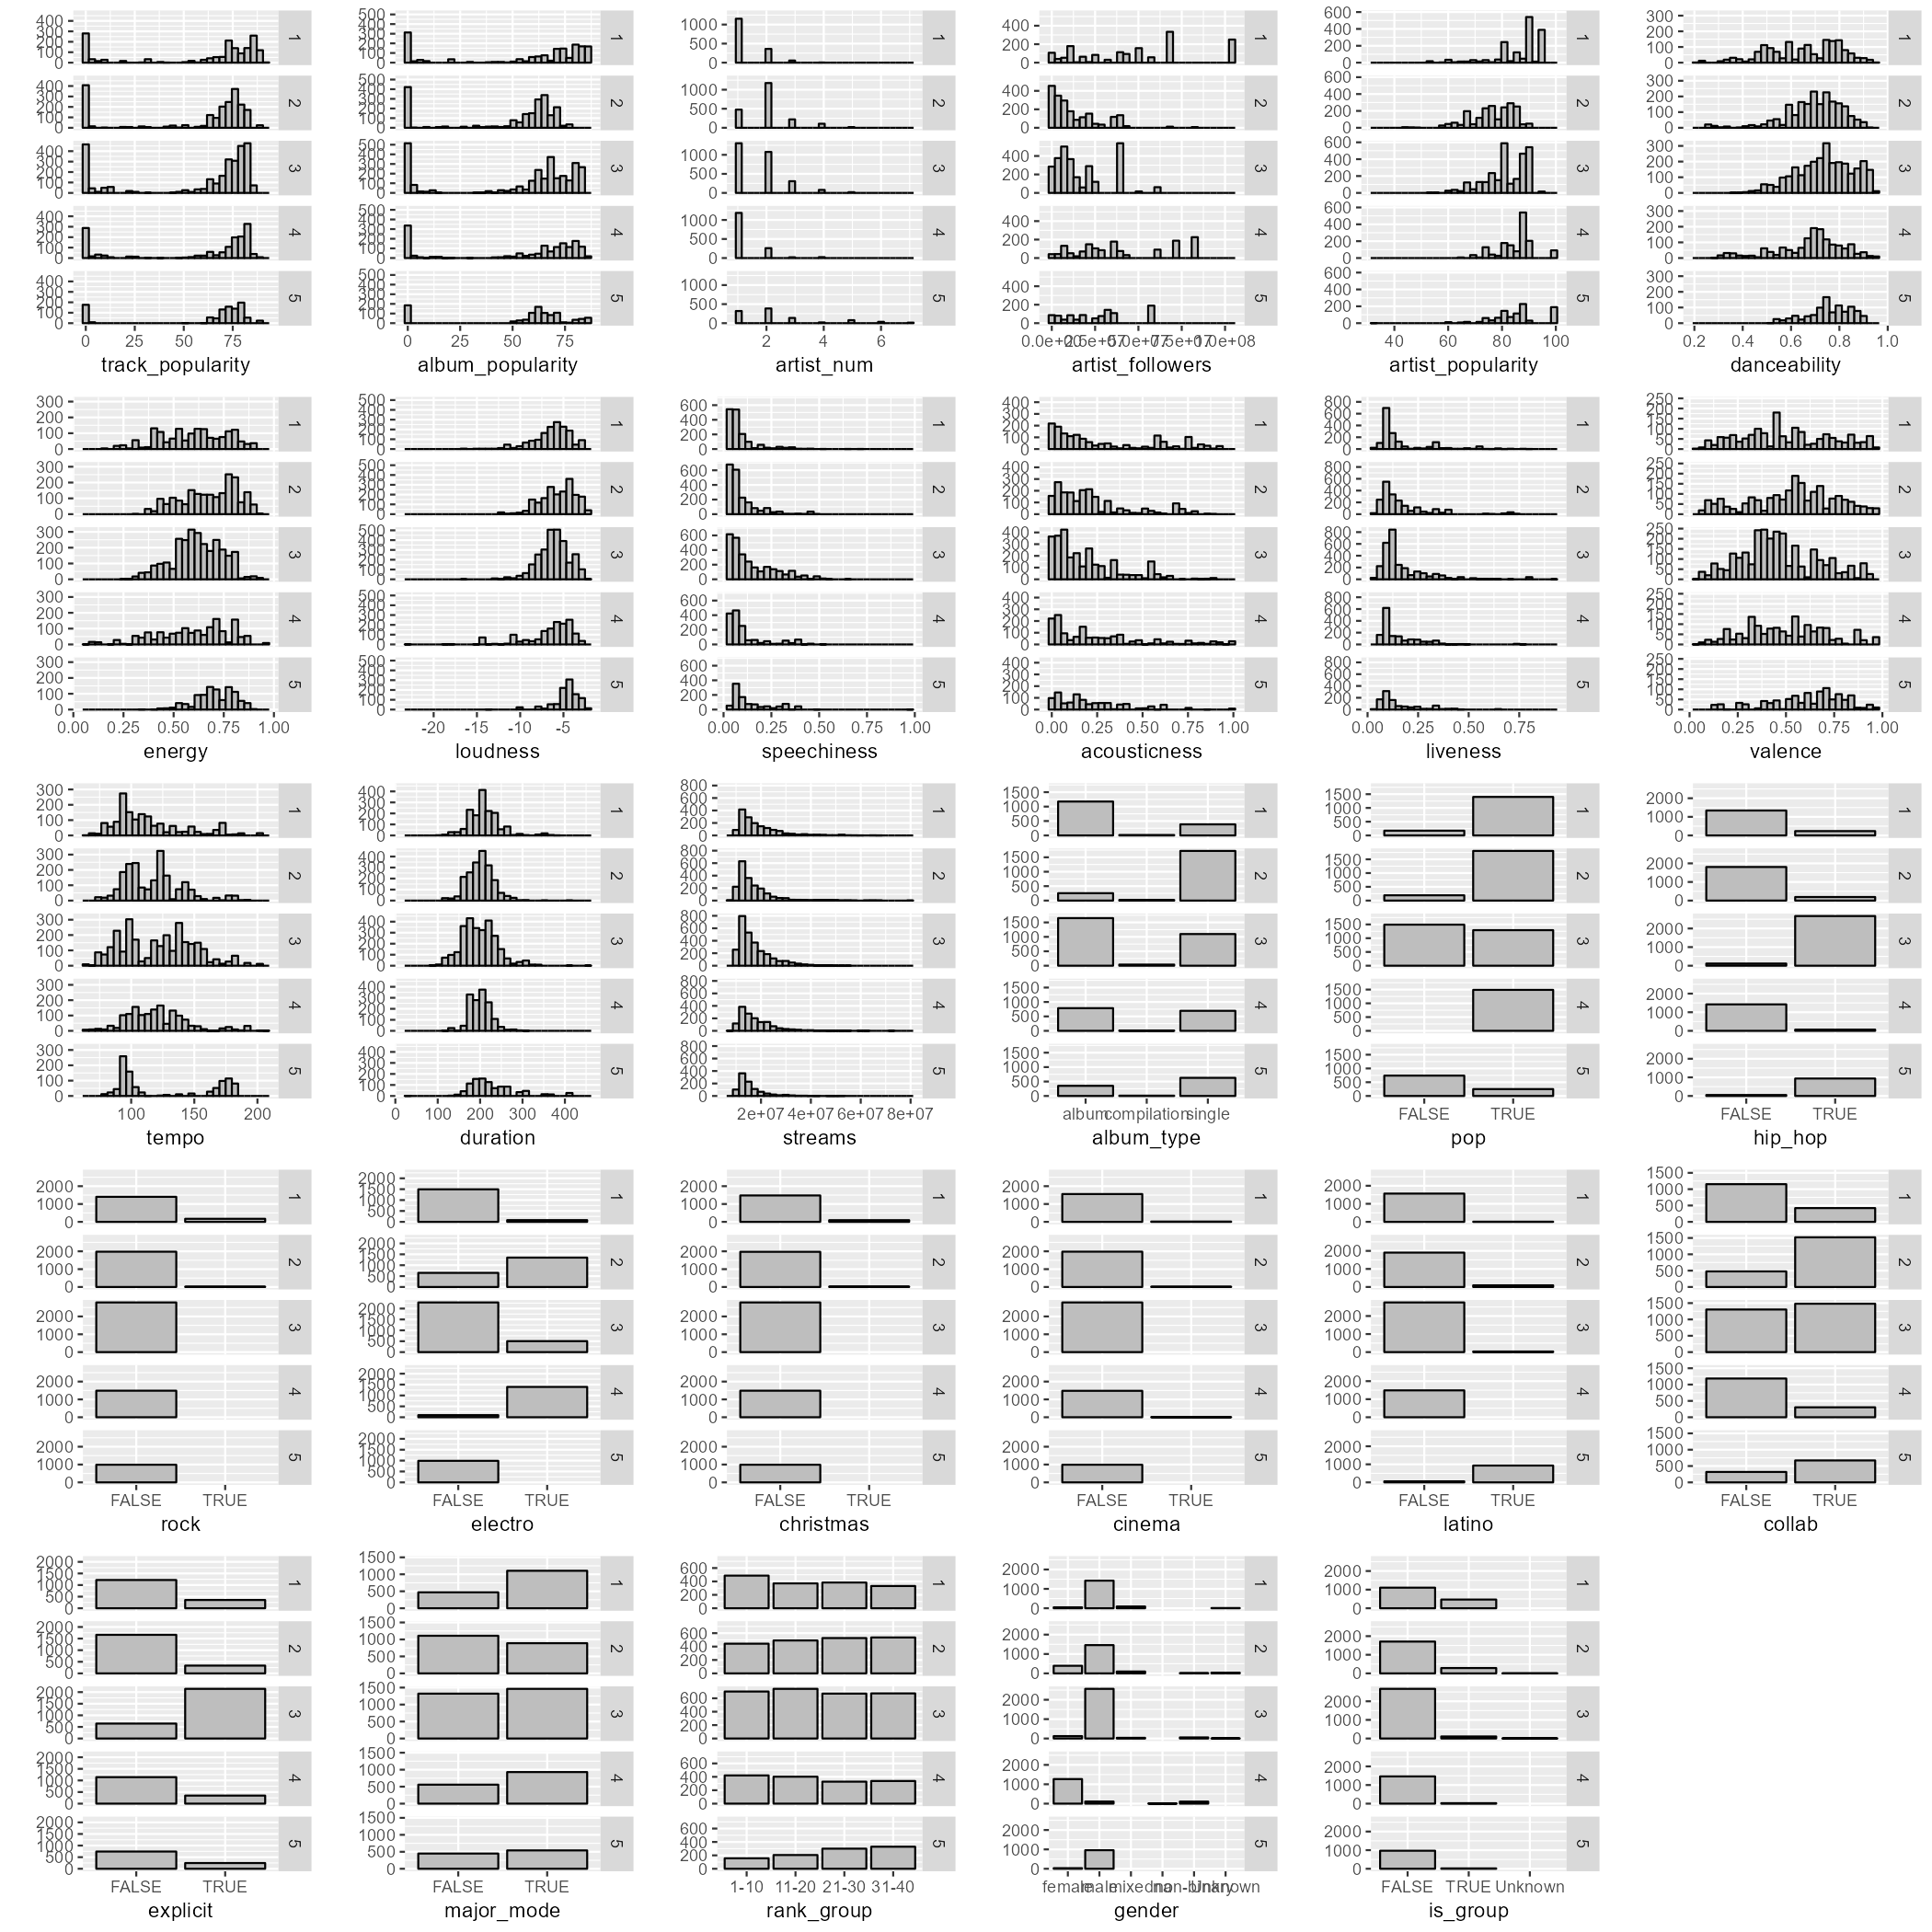
\includegraphics[width=0.96\textwidth]{Images/5_TLP/CPG.png}
    \caption{\emph{Class Panel Graph} inicial}
    \label{fig:5_TLP:CPG_og}
\end{figure}


Per altra banda, en les variables categòriques sí que es poden apreciar diferències més clares. Pel que fa als gèneres, els clusters 1, 2 i 4 són clarament cançons de \textit{pop}, mentre que els 3 i 5 són predominantment de hip\_hop. També es veu que el gènere latino es concentra clarament al 5è grup, i que les cançons explícites s'agrupen al cluster 3.
 
\subsection{Termòmetre}

Una vegada analitzat per sobre el CPG i amb ajuda de les descripcions univariants de les diferents variables (la seva mitjana, moda i els quartils), s'han començat a crear els termòmetres (descrits en \cite{angerri_2023_variable}) que ajudaran a crear un TLP fàcilment interpretable per qualsevol persona. Tot i que els termòmetres haurien de crear-se amb ajuda d'un expert en el camp de la base de dades, com que se'n disposava d'un, s'ha escollit es base al 1r i 3r quartil, com en la forma de la distribució de les variables.

Per crear aquests termòmetres, figures \ref{fig:5_TLP:trackpopularity}-\ref{fig:5_TLP:streams}, s'han separat les variables escollides en l'anterior apartat entre aquelles numèriques i categòriques; ja que els termòmetres de les numèriques i categòriques tenen estructures diferents.

Una vegada separades, per cada variable numèrica s'ha apuntat en una taula d'Excel el seu valor màxim i mínim, i els seus dos límits: que separen el color verd del groc (\textbf{b}), i el groc del vermell (\textbf{a}). El color verd s'ha assignat al conjunt de valors agrupat entre el valor màxim de la variable i la $b$, el vermell al conjunt de dades amb valors de la variable que es trobin entre el mínim i la $a$, i el groc s'ha assignat a les dades amb valors entre la $a$ i la $b$. En la majoria dels casos, per distribució de les variables, s'han apropat molt l'$a$ i la $b$ al primer i tercer quartil.

\begin{figure}[H]
\centering
    \begin{minipage}{.49\textwidth}
        \centering
	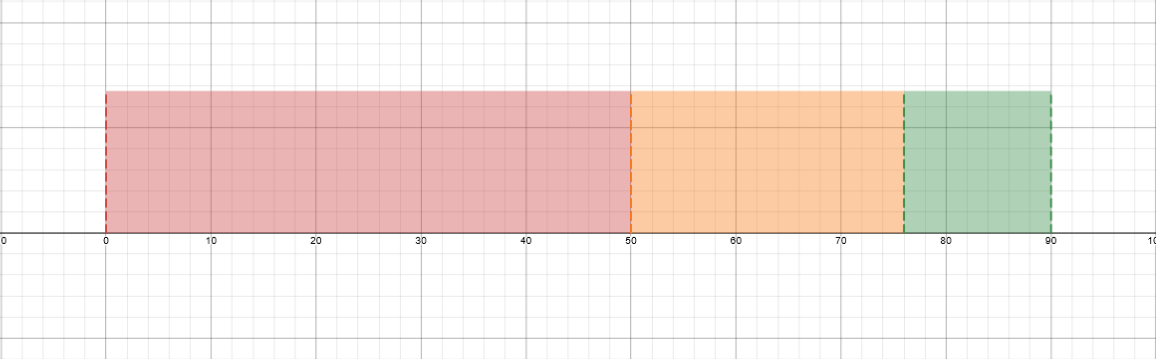
\includegraphics[width=0.95\linewidth]{Images/5_TLP/track_popularity_term.png}
        \caption{Termòmetre de \emph{track\_popularity}}
        \label{fig:5_TLP:trackpopularity}
    \end{minipage}%
    \begin{minipage}{.49\textwidth}
        \centering
        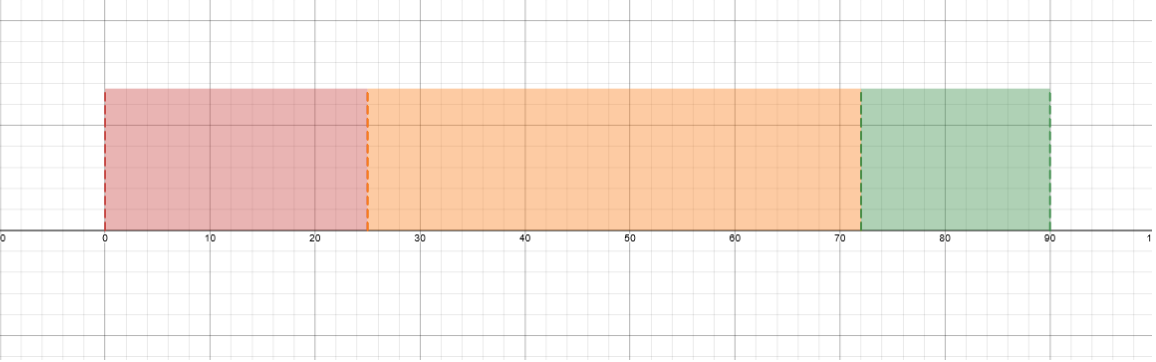
\includegraphics[width=0.95\linewidth]{Images/5_TLP/album_popularity_term.png}
        \caption{Termòmetre de \emph{album\_popularity}}
        \label{fig:5_TLP:albumpopularity}
    \end{minipage}%
\end{figure}

\begin{figure}[H]
\centering
    \begin{minipage}{.49\textwidth}
        \centering
        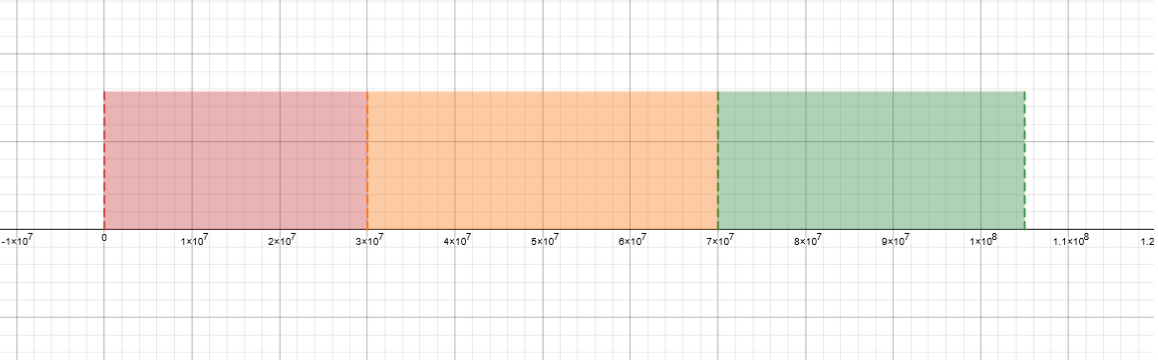
\includegraphics[width=0.95\linewidth]{Images/5_TLP/artist_followers_term.png}
        \caption{Termòmetre de \emph{artist\_followers}}
        \label{fig:5_TLP:artistfollowers}
    \end{minipage}%
    \begin{minipage}{.49\textwidth}
        \centering
        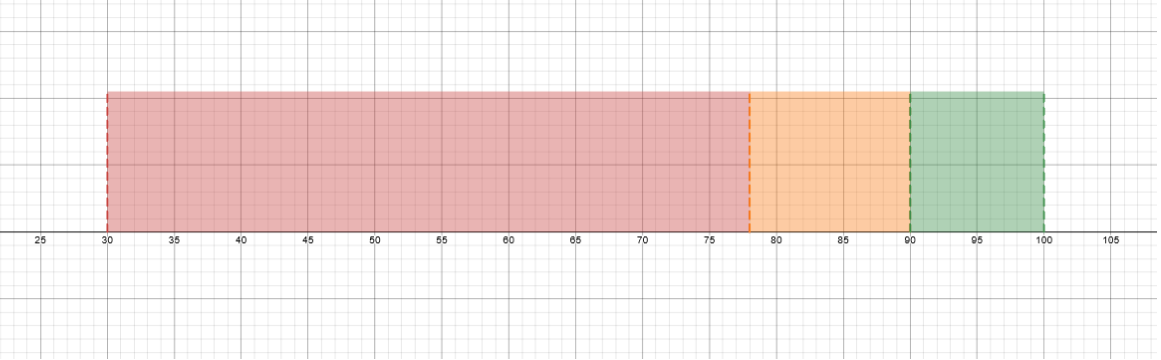
\includegraphics[width=0.95\linewidth]{Images/5_TLP/artist_popularity_term.png}
        \caption{Termòmetre de \emph{artist\_popularity}}
        \label{fig:5_TLP:artistpopularity}
    \end{minipage}%
\end{figure}

\begin{figure}[H]
\centering
    \begin{minipage}{.49\textwidth}
        \centering
        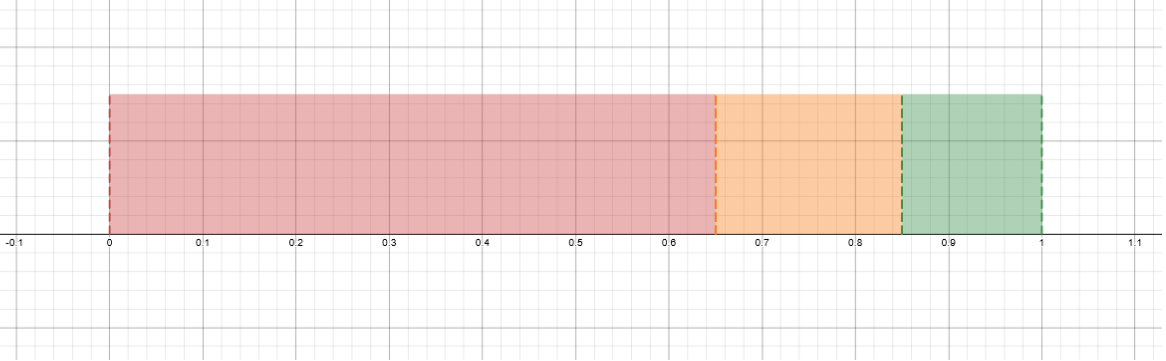
\includegraphics[width=0.95\linewidth]{Images/5_TLP/danceability_term.png}
        \caption{Termòmetre de \emph{danceability}}
        \label{fig:5_TLP:danceability}
    \end{minipage}%
    \begin{minipage}{.49\textwidth}
        \centering
        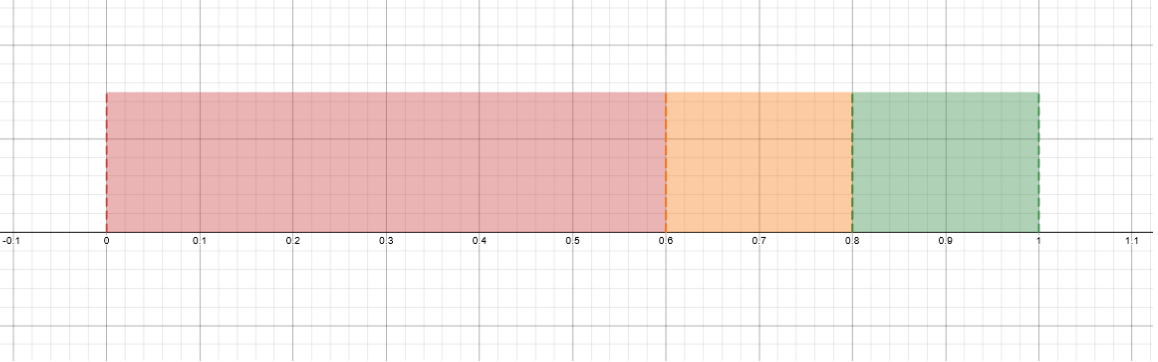
\includegraphics[width=0.95\linewidth]{Images/5_TLP/energy_term.png}
        \caption{Termòmetre de \emph{energy}}
        \label{fig:5_TLP:energy}
    \end{minipage}%
\end{figure}

\begin{figure}[H]
\centering
    \begin{minipage}{.49\textwidth}
        \centering
        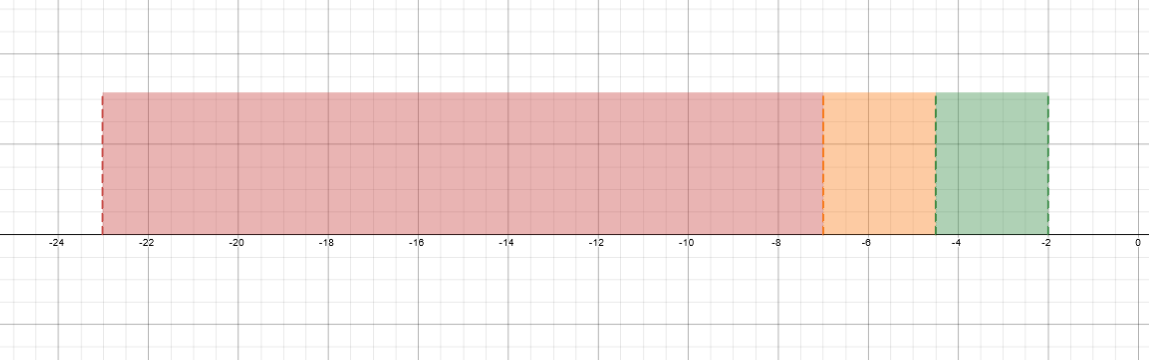
\includegraphics[width=0.95\linewidth]{Images/5_TLP/loudness_term.png}
        \caption{Termòmetre de \emph{loudness}}
        \label{fig:5_TLP:loudness}
    \end{minipage}%
    \begin{minipage}{.49\textwidth}
        \centering
        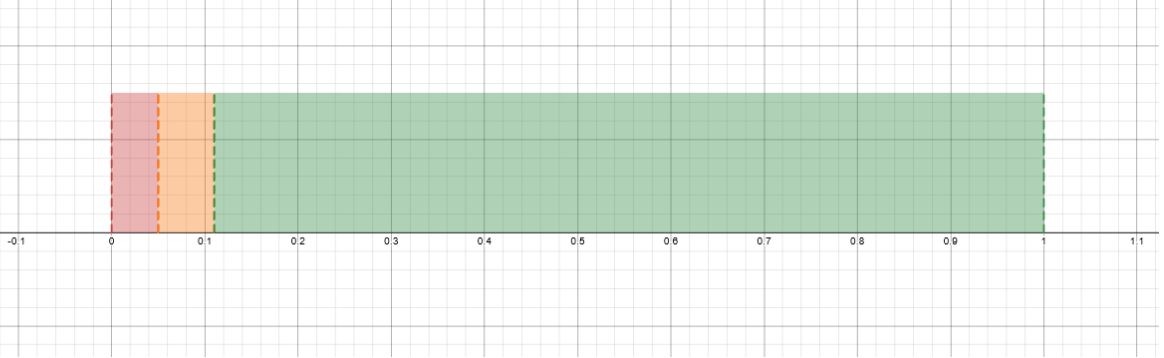
\includegraphics[width=0.95\linewidth]{Images/5_TLP/speechiness_term.png}
        \caption{Termòmetre de \emph{speechiness}}
        \label{fig:5_TLP:speechiness}
    \end{minipage}%
\end{figure}

\begin{figure}[H]
\centering
    \begin{minipage}{.49\textwidth}
        \centering
        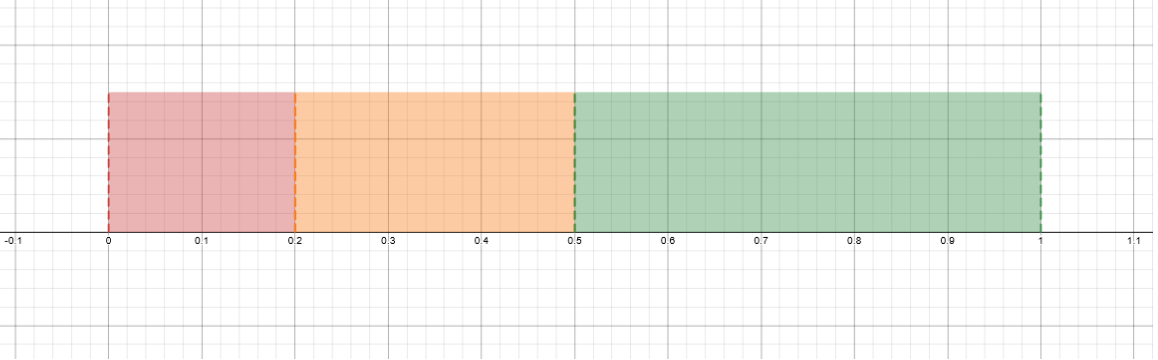
\includegraphics[width=0.95\linewidth]{Images/5_TLP/acousticness_term.png}
        \caption{Termòmetre de \emph{acousticness}}
        \label{fig:5_TLP:acousticness}
    \end{minipage}%
    \begin{minipage}{.49\textwidth}
        \centering
        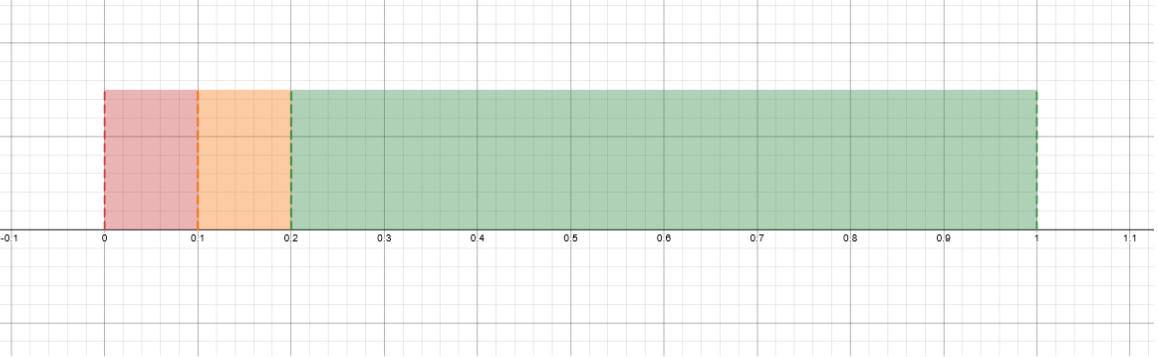
\includegraphics[width=0.95\linewidth]{Images/5_TLP/liveness_term.png}
        \caption{Termòmetre de \emph{liveness}}
        \label{fig:5_TLP:liveness}
    \end{minipage}%
\end{figure}

\begin{figure}[H]
\centering
    \begin{minipage}{.49\textwidth}
        \centering
        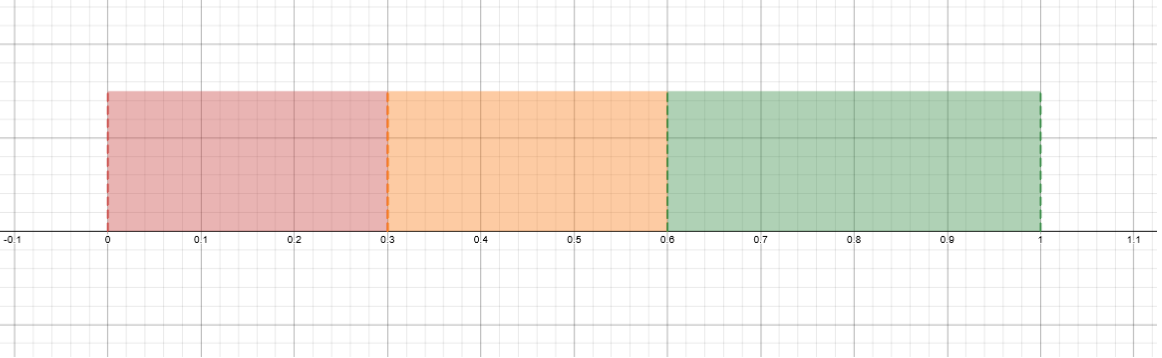
\includegraphics[width=0.95\linewidth]{Images/5_TLP/valence_term.png}
        \caption{Termòmetre de \emph{valence}}
        \label{fig:5_TLP:valence}
    \end{minipage}%
    \begin{minipage}{.49\textwidth}
        \centering
        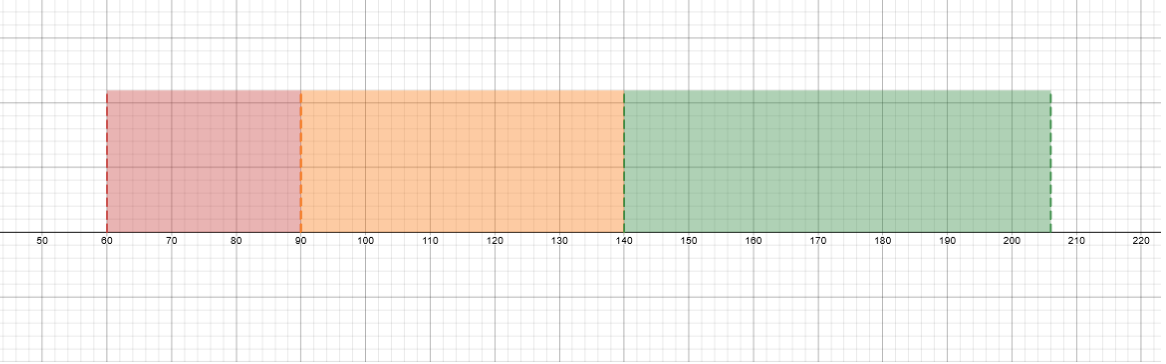
\includegraphics[width=0.95\linewidth]{Images/5_TLP/tempo_term.png}
        \caption{Termòmetre de \emph{tempo}}
        \label{fig:5_TLP:tempo}
    \end{minipage}%
\end{figure}

\begin{figure}[H]
\centering
    \begin{minipage}{.49\textwidth}
        \centering
        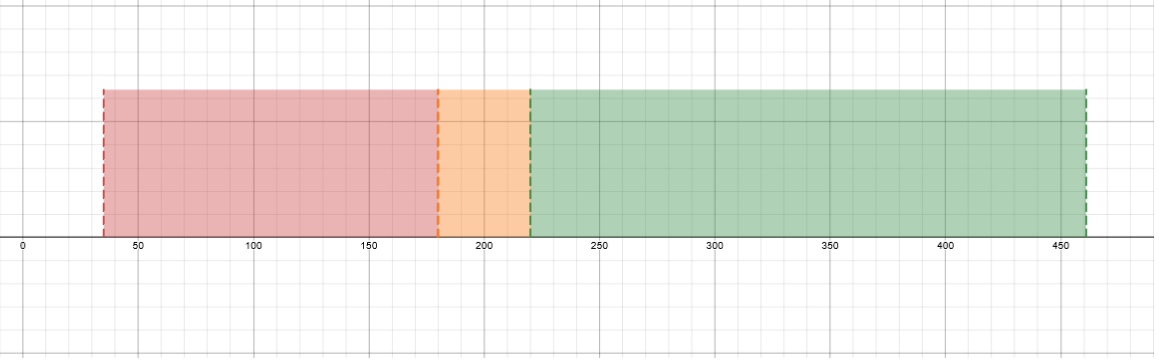
\includegraphics[width=0.95\linewidth]{Images/5_TLP/duration_term.png}

        \caption{Termòmetre de \emph{duration}}
        \label{fig:5_TLP:duration}
    \end{minipage}%
    \begin{minipage}{.49\textwidth}
        \centering
        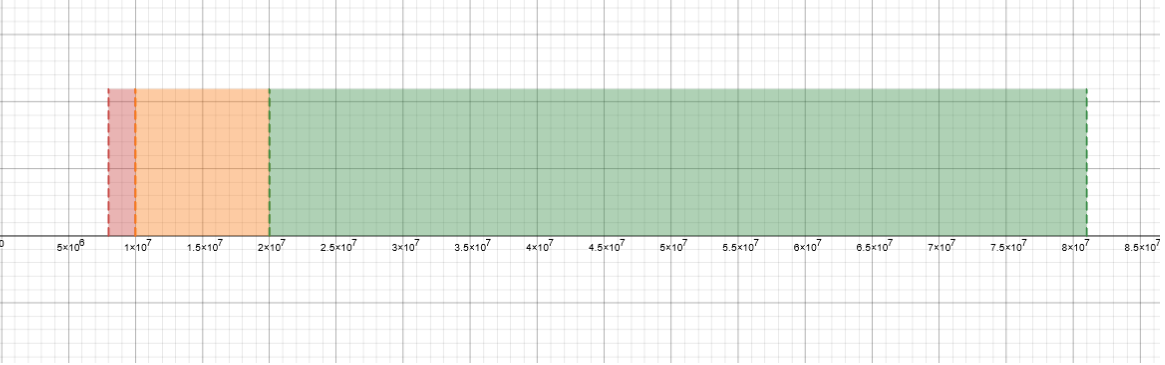
\includegraphics[width=0.95\linewidth]{Images/5_TLP/streams_term.png}
        \caption{Termòmetre de \emph{streams}}
        \label{fig:5_TLP:streams}
    \end{minipage}%
\end{figure}


En el que a les variables categòriques respecta, s'ha classificat cadascuna de les seves modalitats amb el color verd o vermell, fent que aquelles no classificades siguin el color groc. En una altra taula d'Excel s'han apuntat les diferents modalitats que pertanyen al color verd separat per un espai en la columna \textit{green\_vector}, i s'ha fet el mateix per les modalitats vermelles.

Per les variables binàries (els generes de les cançons), s'ha decidit que el valor \textit{TRUE} sigui el relacionat amb el color verd, i el valor \textit{FALSE} amb el vermell. La variable rank\_group ha sigut també senzilla de classificar: de verd la modalitat 1-10 (ja que el millor per un artista és tenir la seva cançó amunt dels rànquings) i de vermell 30-40, que seguiria el pitjor lloc que es pot tenir a la nostra base de dades. Per la variable \textit{gender} es va escollir el gènere femení com a color verd i el masculí com a vermell, en \textit{album\_type} single va ser la modalitat verda i àlbum la vermella. Aquesta codificació es pot comprovar a la figura \ref{fig:5_TLP:term_quali}.

Com es pot comprovar, per molt que l'objectiu del termòmetre sigui representar un conjunt de valors d'una variable com a ''dolents'' i un altre com a ''millor'', en la nostra base de dades això no té gaire sentit; ja que, per exemple, el fet de que una cançó sigui o no del genre hip\_hop, no implica cap sentit de millor o pitjor. Si bé potser coincideix que en variables com \textit{streams} o \textit{popularity}, els valors alts sí que van relacionats amb la idea que una cançó tindrà més èxit (que no vol dir que sigui millor, evidentment això és subjectiu), en la majoria d'elles, no té sentit relacionar el verd amb bo i el vermell amb dolent; sinó que seran colors que facilitaran la interpretació i, en la majoria dels casos, el verd representarà valors alts de la variable (numèriques) o valors \textit{TRUE} (categòriques), el vermell el contrari, i el groc un punt mig.

\begin{figure}[H] 
    \centering
    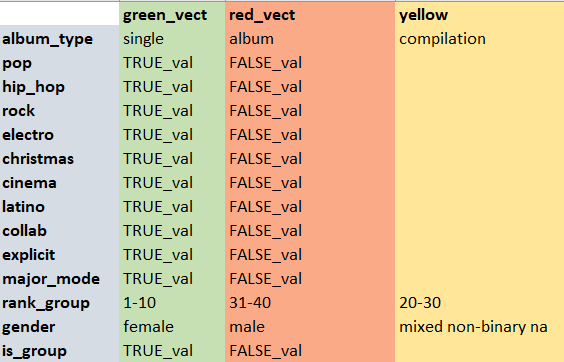
\includegraphics[width=0.7\textwidth]{Images/5_TLP/term_quali.png}
    \caption{Codificació de colors per a les variables categòriques}
    \label{fig:5_TLP:term_quali}
\end{figure}

A continuació, hem creat un petit script de Python que llegirà aquestes taulés d'Excel i les traduirà a una sèrie de llistes de R, escrivint-les dins del script que utilitzarem per crear un pseudo-TLP.

\subsection{pseudo-TLP a partir de termòmetre}

Tenint ja preparats els valors $a$ i $b$ que delimitaran la regió verda de la groga i la groga de la vermella en les variables numèriques, i els colors assignats a cada modalitat en les variables categòriques, hem creat un pseudo-TLP. Aquest pseudo-TLP és un CPG on pintem del seu color corresponent cada subplot per cada variable en cada cluster.

En el cas de les variables numèriques, s'ha escollit el color corresponent de cada subplot utilitzant la mediana. És a dir, es calcula la mediana de cada variable dins del primer, segon, tercer, quart i quint cluster. A continuació, es mira on quedaria aquest valor dins del termòmetre, i s'escull aquest color pel subplot d'aquesta variable amb el cluster corresponent. Aquesta tècnica és bastant robusta a distribucions amb cues molt llargues o amb outliers molt distants, ja que aquests fenòmens faran que la mitjana no caigui en la zona on més valors tindrem, mentre que la mediana, en canvi, caurà on estiguin la majoria dels valors. Tot i això, aquesta mesura fallarà en cas d'aplicar-la amb distribucions bimodals, una cosa que s'haurà de tindre en compte.

Per una altra banda, les variables categòriques han sigut classificades mitjançant l'ús de la moda. D'aquesta manera, en cas d'una variable binomial com \textit{pop}, que conté més valors \textit{TRUE} que \textit{FALSE} en el cluster 1, el color assignat a aquest cluster amb la variable \textit{pop} serà verd.

Tot i així, aprofitant que en les variables binomials no s'està utilitzant el color groc, s'ha decidit crear una petita variació del termòmetre explicat a classe, basat en el següent pensament: el fet que hi hagi més instàncies d'una modalitat que de l'altre, no implica que aquesta sigui predominant del tot dins de la classe, ja que es pot donar el cas que hi hagi 300 \textit{TRUE}s i 289 \textit{FALSE}s, implicant que, realment, no n'hi ha una gran diferència dins d'aquesta variable. Així doncs, s'ha escollit un llindar tal que si la diferència d'instàncies entre les dues modalitats predominants (les més freqüents) d'una variable és menor d'aquest llindar, el color de la variable en aquest cluster sigui groc. En cas de variables amb més de dues modalitats, no s'ha implementat a tot i ara el color groc pot tenir dos significats: o bé pertany a una classe groga, o les seves dues modalitats principals es reparteixen de manera prou uniforme.
\begin{figure}[H] 
    \centering
    \includegraphics[width=0.96\textwidth]{Images/5_TLP/TLP.png}
    \caption{pseudo-\emph{Traffic Light Panel} inicial}
    \label{fig:5_TLP:TLP_og}
\end{figure}

Havent aplicat ja aquestes regles amb tal d'escollir els diferents colors, ens ha quedat el següent pseudo-TLP: figura \ref{fig:5_TLP:TLP_og}. Tal com es pot apreciar, en les variables numèriques tenim certes diferències tant en artist\_num com en artist\_followers, tal com s'ha vist al profiling clàssic. Tot i això, a diferència de les conclusions del profiling anterior, artist\_popularity també té una moda i distribució diferent d'aquelles dels clusters 1, 3, 4 i 5 al cluster número 2, implicant artistes una mica menys populars dins d'aquest clusters. Loudness té una petita diferència de moda, ja que la distribució del cluster 5 té una cua esquerra menys curta que la resta de distribucions a les altres classes, implicant cançons una mica més sorolloses. La variable valence també una moda diferent, tot i que la distribució no canvia tant, degut principalment a què la moda es troba just al límit entre els colors verd i groc del seu semàfor (el límit seguint 0.6 i la moda 0.656). Finalment, la resta de variables no tenen cap diferència significant en el que a la moda o distribució respecta. Cal comentar que la variable tempo no té cap diferència de color degut, probablement, a la distribució binomial que té.

Per altra banda, mirant les variables categòriques, trobem les mateixes conclusions en la variable album\_type, amb més àlbums als clusters 1 i 3, més singles als clusters 2 i 5, i quasi cap diferència al 4. Respecte als gèneres musicals, pop es concentra en les clases 1, 2 i 4, mentre que hip\_hop es concentra en les classes oposades. Electro coincideix als clusters 2 i 4 amb pop i latino es troba al cluster 5. Rock, christmas i cinema no són predominants en cap cluster, trobant-se així totes de color vermell. La variable collab es concentra en els clusters 2 i 5, mentre que en el 3 existeix un repartiment proporcional d'ambdues modalitats. Explicit es concentra al cluster 3, major\_mode a l'1 i 4 però amb un repartiment bastant equitatiu, i rank\_group es divideix de manera molt uniforme. Finalment, cal destacar que les artistes de gener femení es troben al cluster 4 i que is\_group és sempre majoritàriament \textit{FALSE}.

\subsection{TLP final}

Una vegada analitzats els resultats del pseudo-TLP complet i basant-nos en el treball fet al profiling clàssic, tal com es menciona en l'article on s'explica detalladament el TLP, s'haurien de treure les variables que no aporten cap informació a les classes en un TLP final, per tal de fer-lo encara més interpretable del que ja és. Així doncs, s'ha decidit treure les variables que ni al pseudo-TLP previ (figura \ref{fig:5_TLP:TLP_og}) ni al profiling clàssic han aportat cap mena de variància. Aquestes són: track\_popularity, album\_popularity, liveness, tempo, duration, cinema, rock i cinema. Eliminant aquestes variables, s'ha obtingut el següent pseudo-TLP (figura \ref{fig:5_TLP:TLP_red}) i s'ha procedit a construir el TLP final.

\begin{figure}[H] 
    \centering
    \includegraphics[width=0.96\textwidth]{Images/5_TLP/TLP_reduced.png}
    \caption{TLP amb variables reducides}
    \label{fig:5_TLP:TLP_red}
\end{figure}

Finalment, si seguim al peu de la lletra les instruccions i introduïm els colors dins d'una taula d'Excel, la figura \ref{fig:5_TLP:TLP_final} seguiria el nostre TLP final.

\begin{figure}[H] 
    \centering
    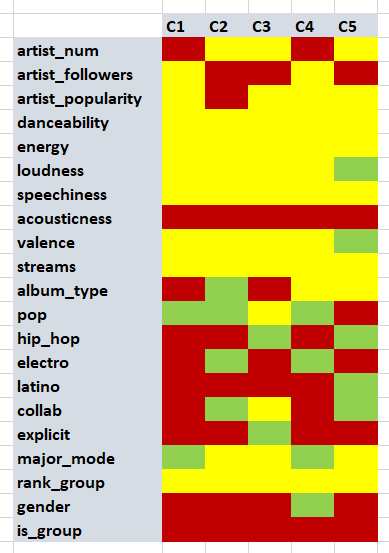
\includegraphics[width=0.66\textwidth]{Images/5_TLP/TLP_final.png}
    \caption{TLP final}
    \label{fig:5_TLP:TLP_final}
\end{figure}